\documentclass[12pt,onecolumn,a4paper,fleqn]{article}
\usepackage{epsfig,graphicx,subfigure,amsthm,amsmath}
\usepackage[table,xcdraw,svgnames]{xcolor}
\usepackage{mathtools}
\usepackage{fancyhdr}
\usepackage{sidecap}
\usepackage{tikz}
\usepackage{pgfplots}
\usetikzlibrary{decorations.pathreplacing}
\usepackage{relsize}
\usepackage{color,xcolor}
\usepackage[framed,numbered]{matlab-prettifier}
\usepackage{files/persianheader}     
\usepackage{float}
\usepackage{enumerate}
\usepackage{booktabs}
\usepackage{xepersian}


\settextfont[Path=fonts/,BoldFont={ZarBd.ttf},BoldFeatures={Scale=0.9}]{BZar.ttf}

\DeclarePairedDelimiter\ceil{\lceil}{\rceil}
\DeclarePairedDelimiter\floor{\lfloor}{\rfloor}


\pagestyle{fancy}
\fancyhf{}
\rhead{\textbf{طراحی سیستم‌های دیجیتال}}
\chead{\textbf{گزارش پروژه}}
\lhead{\textbf{\nouppercase{\rightmark}}}
\cfoot{({\thepage})}
\renewcommand{\headrulewidth}{1pt}
\renewcommand{\footrulewidth}{1pt}
\renewcommand{\sectionmark}[1]{\markright{#1}}
\renewcommand{\subsectionmark}[1]{\markright{#1}}


\begin{document}
%%% title pages
\large
\begin{titlepage}
	
	\begin{center}
		\begin{Large}
			\textbf{
				به نام خدا\\
			}
		\end{Large}
		
		\vspace{2cm}
		
\includegraphics[scale=0.6]{files/sharif-logo.png}\\
		\vspace{0.5cm}
		\begin{Large}
			\textbf{
				دانشگاه صنعتی شریف\\
				\vspace{0.5cm}
				دانشکده مهندسی کامپیوتر\\
			}
		\end{Large}
		\vspace{2.5cm}
		\begin{huge}
			\textbf{
				طراحی سیستم‌های دیجیتال\\
				\vspace{0.5cm}
			}
		\end{huge}
		
		\begin{Large}
			\textbf{
				پروژه‌ی پایانی درس:\\ ضرب‌کننده‌ی ماتریسی با استاندارد \lr{IEEE 754} \\
			}
		\end{Large}
		
		\noindent\rule[1ex]{\linewidth}{1pt}
		\vspace{1.5cm}
		\begin{Large}{
				استاد:
				\textbf{
					دکتر فرشاد بهاروند \\
				}
				عماد زین‌اوقلی، مازیار شمسی‌پور، بردیا محمدی، جواد هزاره، پویا یوسفی
				
				\vspace{1.5cm}
				\textbf{\today}
			}
		\end{Large}
		
	\end{center}
	\thispagestyle{empty}
\end{titlepage}	

\pagebreak

\tableofcontents
\thispagestyle{empty}
\pagebreak


\section*{شرح وظایف}
\markright{شرح وظایف}


\pagebreak



\section{مقدمه}
	
	\subsection{تعریف الگوریتم}
	الگوریتم مورد استفاده الگوریتم ضرب ماتریسی \lr{Cannon} می‌باشد در این الگوریتم با تقسیم کردن ماتریس‌های ورودی و خروجی به بلاک‌های $k*k$ که در آن $k$ عدد ثابتی می‌باشد می‌خواهیم با داشتن تعدادی پردازنده‌ که به صورت موازی کار می‌کنند عملیات ضرب ماتریسی را بهبود ببخشیم. به طور مثال ماتریس‌ها زیر را در نظر بگیرید:
	\begin{equation}
	A = \begin{bmatrix}
	A_{11}& A_{12}& \dots A_{1\mu}\\
	\vdots& \ddots& \vdots\\
	A_{\lambda1}& A_{\lambda2}& \dots A_{\lambda\mu}\\
	\end{bmatrix} 
	\ \ \, 
	B = \begin{bmatrix}
	B_{11}& B_{12}& \dots B_{1\gamma}\\
	\vdots& \ddots& \vdots\\
	B_{\mu1}& B_{\mu2}& \dots B_{\mu\gamma}\\
	\end{bmatrix} 
	\end{equation}
	
	که در آن هر $A_{ij} و B_{ij}$ یک بلاک $k*k$ می‌باشد.(توجه می‌کنیم که  سایز‌ ماتریس‌ها اگر بخش‌‌پذیر به $k$ نباشد با اضافه‌ کردن صفر آن را بخش پذیر می‌کنیم) با این اوصاف طبق قاعده‌ی ضرب بلوکی می‌دانیم که بلاک $C_{ij}$ در ماتریس جواب از رابطه‌ی زیر محاسبه می‌شود.
	\begin{equation}
	C_{ij} = \sum_{x=0}^\mu A_{ix}B_{xj}
	\label{1}
	\end{equation}
	
	با داشتن تعداد تعداد مشخصی ضرب کننده‌ی ماتریسی $k*k$ می‌توانیم  به طور موازی با استفاده از آنها  و پخش ‌کردن $C_{ij}$ ها بین پردازنده‌های مختلف حاصل نهایی $A\times B$ را محاسبه کنیم. 

در ادامه‌ی این گزارش از علائم ریاضی‌ای استفاده می‌شود که در اینجا به شرح‌ آنها می‌پردازیم.
	
\subsection{قرارداد‌های ریاضی}

ورودی الگوریتم مورد استفاده  ماتریس‌های مستطیلی $A_{mr}$ و $B_{rn}$ خواهند بود و بنابراین ماتریس‌ خروجی به صورت
$A_{mr} \times B_{rn} = C_{mn}$
خواهد بود. با این‌ حال در هر کجای گزارش که از عبارت $A_{ij}$ (و همینطور برای $B,C$) استفاده شد منظور بلاک‌ $k*k$ ستون $i$ام و سطر $j$ام می‌باشد. برای روشن‌تر شدن این موضوع به مثال زیر توجه می‌کنیم، فرض کنید ماتریس $A$ به صورت زیر باشد:

	$$ A_{mr} = \begin{bmatrix}
	a_{00}& a_{01}& \dots& a_{0r}\\
	\vdots& \vdots& \ddots& \vdots\\
	a_{m0}& a_{m1}& \dots& a_{mr}
	\end{bmatrix} $$
	
	حال اگر این ماتریس را به بلوک‌های $k*k$ تقسیم کنیم و در صورت لزوم درایه‌های نهایی را صفر قرار دهیم ماتریسی به فرم زیر خواهیم داشت:
	
	$$ A^* = \begin{bmatrix}
	\begin{array}{cccc|c}
		A_{00} & A_{01} & \dots & A_{0\mu-1} &  \\
		\vdots & \vdots & \ddots & \vdots & 0 \\
		A_{\lambda-10} & A_{\lambda-11} & \dots & A_{\lambda\mu-1} & \\
		\hline
			& 0 & & & 0
	\end{array}
	\end{bmatrix} $$
که لازم است که توجه داشته باشیم که وقتی ماتریس‌ها را به فرم بلوکی می‌نویسیم مقادیر زیر را تعریف می‌کنیم:
\begin{subequations}
	\begin{equation}
		\mu = \ceil*{\dfrac{r}{k}}
	\end{equation}    
	\begin{equation}
		\lambda = \ceil*{\dfrac{m}{k}}
	\end{equation}
	\begin{equation}
		\gamma = \ceil*{\dfrac{n}{k}}
	\end{equation}
	\label{2}
\end{subequations}
از این نماد‌ها به کرّات در طول گزارش استفاده خواهد شد. توجه می‌کنیم که علت اینکه سقف این حاصل تقسیم‌ها را در نظر گرفتیم همان است که اگر اندازه‌ی ماتریس‌ها بر $k$ بخش‌پذیر نباشند با اضافه کردن صفر به انتها‌ی آن باعث بخش‌پذیری می‌شویم. 
\subsection{نحوه‌ی عملکرد از نظر مساحت و تایمینگ}
از آنجایی که هر ضرب کننده‌ی ماتریسی در حدود
 $k^3$
 کلاک سایکل زمان می‌برد و محاسبه‌ی هر بلوک $C_{ij}$ با توجه به
 \autoref{1}
به $\mu$ بار به ضرب ماتریسی نیاز دارد. همچنین برای محاسبه‌ی تمام بلوک‌ها باید $\lambda\gamma$ بار محاسبات بالا را انجام دهیم با این حال اگر فرض کنیم که تعداد پردازنده‌ها $p$ باشد آنگاه می‌توانیم ببینیم که تعداد کلاک‌ سایکل‌ها تقریبا برابر با عبارت زیر است:
\begin{equation}
	\dfrac{\lambda\gamma\mu k^2}{\text{\lr{\#number of PU}}} = 	\dfrac{\lambda\gamma\mu k^2}{p}
\end{equation}

همچنین تعداد رجیستر‌هایی که هر واحد ضرب‌کننده‌ی ماتریس مربعی نیاز دارد از $O(k^2)$ می‌باشد. و بنابراین تعداد تمام رجیستر‌هایی که مورد نیاز است از $O(pk^2)$ می‌باشد.

	\pagebreak

\subsection{استاندارد‌ \lr{IEEE 754}}
محاسبات در این پروژه از استاندارد
 \lr{IEEE 754 - Single-precision floating-point}
 پیروی می‌کند که به طور مختصر به شرح آن می‌پردازیم. \\
 در این استاندارد اعداد اعشار با سه بخش \lr{exponent} , \lr{fraction} , \lr{sign} مشخص می‌شوند که سهم هر یک از آنها مانند مثال زیر است:
 
\begin{figure}[h]
	\centering
	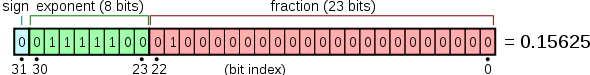
\includegraphics[width=0.8\linewidth]{source/float_example.png}
\end{figure}

و هر عدد طبق فرمول زیر به این نمایش در می‌آید:

\begin{equation}
\text{value} = (-1)^{sign} \times 2^{(E-127)} \times (1 + \sum_{i=1}^{23}b_{23-i}2^{-i})
\end{equation}
 
 \pagebreak

\subsection{مراجع مورد استفاده}

\begin{latin}
\begin{thebibliography}{}
	
	\bibitem{parallel} 
	Abhishek Kumar : Scalability of Parallel Algorithms for Matrix Multiplication
	
	\bibitem{parallel} 
	Patricia Ortega : Parallel Algorithm for Dense Matrix Multipication
	
	\bibitem{area} 
	Ju-wook Jang, Seonil Choi and Viktor K. Prasanna : Area and Time Efficient Implementations of Matrix Multiplication on FPGAs
	
	\bibitem{cannon}
	Cannon's algorithm, Wiki-pedia\\ https://en.wikipedia.org/wiki/Cannon\%27s\_algorithm
	
	
\end{thebibliography}
\end{latin}

\pagebreak

\section{توصیف معماری سیستم}
\subsection{اینترفیس‌های سیستم و قرارداد استفاده از آن }
به طور کلی سخت‌افزار از یک حافظه و بخش محاسبه‌ی ضرب ماتریسی تشکیل شده است که پردازنده‌ می‌تواند ورودی‌ها را درون حافظه قرار داده و خروجی‌ها را نیز از آن بخواند.
(\lr{I/O Map}). 
با این حال قرارداد‌هایی در نحوه‌ی استفاده از مموری وجود دارد که باید به آن توجه شود. ساختار کلی حافظه به صورت زیر خواهد بود:
\vspace{3cm}
\begin{table}[h]
	\centering
	\begin{tabular}{clll}
		\hline
		\multicolumn{4}{|c|}{Config}                                          \\ \hline
		\multicolumn{4}{|c|}{Status}                                          \\ \hline
		\multicolumn{4}{|c|}{$A_{11}$}                                        \\ \hline

		\multicolumn{4}{|c|}{$A_{12}$}                                        \\ \hline

		\multicolumn{4}{|c|}{$\vdots$}                                        \\ \hline
		\multicolumn{4}{|c|}{$A_{\lambda\mu}$}  \\ \hline   
		\multicolumn{4}{|c|}{$B_{11}$}                                        \\ \hline
		\multicolumn{4}{|c|}{$B_{12}$}                                        \\ \hline
				\multicolumn{4}{|c|}{$\vdots$}                                        \\ \hline
		\multicolumn{4}{|c|}{$B_{\mu\gamma}$}                                        \\ \hline
				\multicolumn{4}{|l|}{\cellcolor[HTML]{595959}{\color[HTML]{595959}aaaaaaaaaaaaaaaaaaaaa }} \\ \hline   
			\multicolumn{4}{|c|}{$C_{11}$}                                        \\ \hline
	
	\multicolumn{4}{|c|}{$C_{12}$}                                        \\ \hline
	
	\multicolumn{4}{|c|}{$\vdots$}                                        \\ \hline
	\multicolumn{4}{|c|}{$C_{\lambda\gamma}$}  \\ \hline 
	    				\multicolumn{4}{|l|}{\cellcolor[HTML]{595959}{\color[HTML]{595959}aaaaaaaaaaaaaaaaaaaaa }} \\ \hline   
	\end{tabular}
	\caption{شماتیک حافظه}
\end{table}

\pagebreak

که در آن هر یک از $A_{ij} , B_{ij} , C_{ij}$ها یک بلوک $k*k$ خواهند بود و باید آن‌ها را به صورت سطری در خانه‌های پشت سر هم حافظه نوشت. برای مثال اگر ماتریس $A$ به صورت زیر باشد:
$$ A = \begin{bmatrix}
1& 2 & 3\\
4& 5 & 6
\end{bmatrix} $$

و در صورتی که 
$k=2$
و به عبارتی بلوک‌ها $2*2$ باشند \lr{CPU} باید آن را به صورت زیر در حافظه قرار دهد:

\begin{table}[h]
	\centering
	\begin{tabular}{clll}
		\hline
		\multicolumn{4}{|c|}{Config}                                          \\ \hline
		\multicolumn{4}{|c|}{Status}                                          \\ \hline
		\multicolumn{4}{|c|}{1}                                        \\ \hline
		\multicolumn{4}{|c|}{2}                                        \\ \hline
		\multicolumn{4}{|c|}{4}                                        \\ \hline
		\multicolumn{4}{|c|}{5}                                        \\ \hline
		
		\multicolumn{4}{|c|}{3}                                        \\ \hline
				\multicolumn{4}{|c|}{0}                                        \\ \hline
					\multicolumn{4}{|c|}{6}                                        \\ \hline
										\multicolumn{4}{|c|}{0}                                        \\ \hline
				\multicolumn{4}{|c|}{$\vdots$}                                        \\ \hline
		\multicolumn{4}{|l|}{\cellcolor[HTML]{595959}{\color[HTML]{595959}aaaaaaaaaaaaaaaaaaaaa }} \\ \hline   
	\end{tabular}
 	\caption{شماتیک حافظه برای مثال داده‌ شده}
\end{table}

به عبارتی وظیفه‌ی بلوک کردن ماتریس و همچنین صفر قرار دادن خانه‌های اضافی به عهده‌ی \lr{CPU} خواهد بود. \\ 
همچنین \lr{CPU} باید اولین خانه‌ی حافظه را که مربوط به کانفیگ می‌باشد به صورت زیر از اعداد پر کند:

\begin{table}[h]
	\centering
	\begin{tabular}{cccc}
		\hline
		\multicolumn{1}{|c|}{$\lambda$} & \multicolumn{1}{c|}{$\gamma$} & \multicolumn{1}{c|}{$\mu$} & \multicolumn{1}{c|}{$\theta$} \\ \hline
		$\overbrace{8 \ bits}$ & $\overbrace{8 \ bits}$             & $\overbrace{8 \ bits}$ & $\overbrace{8 \ bits}$                     
	\end{tabular}
\end{table}

که مقادیر این پارامتر‌ها در 
\autoref{2}
مشخص شده است و البته باید توجه داشته باشید که مقدار $\theta$ نیز از رابطه‌ی زیر محاسبه می‌شود:
\begin{equation}
	\theta = \dfrac{\lambda\gamma}{\text{\lr{\#Matrix Processors}}}
\end{equation}

همچنین دومین خانه‌ی حافظه که مربوط به \lr{Status} می‌باشد مطابق شکل زیر می‌باشد.

\begin{table}[h]
	\centering
	\begin{tabular}{|c|c|c|c|c|}
		\hline
		\lr{CPU Ready} & \lr{MP Acknowledge} & $\dots$ &\lr{CPU Acknowledge} & \lr{MP Ready}\\ \hline
	\end{tabular}
\end{table}
وظیفه‌ی \lr{CPU} این است که بعد از قرار دادن ورودی‌ها و تنظیم کردن \lr{Config} مقدار بیت \lr{CPU Ready} را فعال کند و بعد از این که بیت \lr{Acknowledge} را از طرف ضرب کننده‌ی ماتریسی دریافت کرد به کارش ادامه دهد بعد از تمام شدن عملیات ماتریسی بیت \lr{MP Ready} فعال می‌شود و \lr{CPU} می‌تواند بلاک‌های ماتریس خروجی را از مکانی که در مموری مربوط به خروجی‌ها می‌باشد استخراج کند.

با این تفاسیر تنها ورودی لازم به سخت‌افزار ریست آسنکرون می‌باشد. و با استفاده از مموری سخت‌‌افزار می‌تواند ورودی‌ها را از حافظه خوانده و آنها‌ را محاسبه کند.
\subsection{کلاک سخت‌‌افزار}
تمامی ماژول‌های این سخت‌افزار از جمله مموری و تمام ماژول‌های واحد حساب‌کننده‌ی ضرب ماتریسی به صورت سنکرون عمل می‌کنند و \lr{CDC} در این سخت‌افزار اتفاق نمی‌افتد.

\subsection{دیاگرام‌های بلوکی سخت‌افزار}
این سخت افزار شامل ماژول‌های زیر می‌باشد:
\begin{itemize}
	\item 
	\lr{Memory}
	\item 
	\lr{Arbiter}
	\item 
	\lr{Main Control Unit}
	\item 
	\lr{Control Unit}
	\item 
	\lr{Processor Unit}
	\item 
	\lr{Matrix Multiplier}
	\item 
	\lr{Matrix Adder}
	\item 
	\lr{Index To Address Transformer}
\end{itemize}

	در اینجا به توصیف ورودی‌ خروجی‌ هر یک از آن‌ها و نحوه‌ی اتصال ‌آنها می‌پردازیم و در بخش بعد نحوه‌ی عملکرد هر یک را توضیح می‌دهیم:
	
\begin{figure}[h]
	\centering
	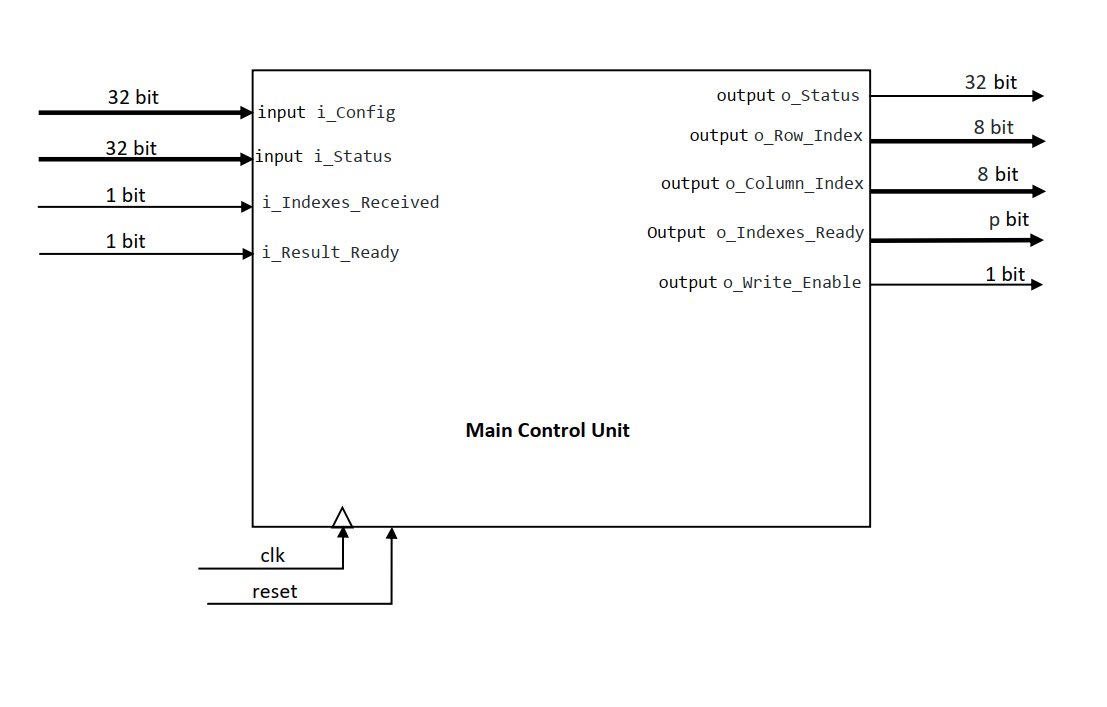
\includegraphics[width=0.5\linewidth]{source/main_cu.png}
	\caption{\lr{Main Control Unit}}
\end{figure}

\begin{figure}[h]
	\centering
	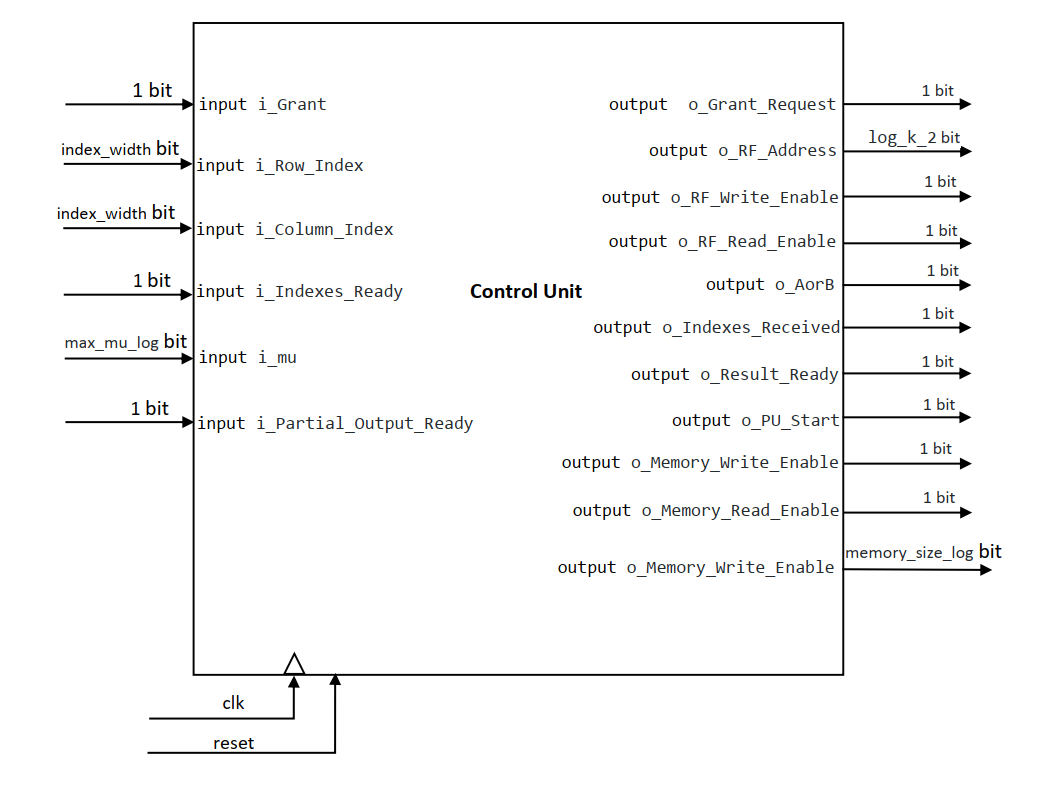
\includegraphics[width=0.5\linewidth]{source/ControlUnit.png}
	\caption{\lr{Control Unit}}
\end{figure}

\begin{figure}[h]
	\centering
	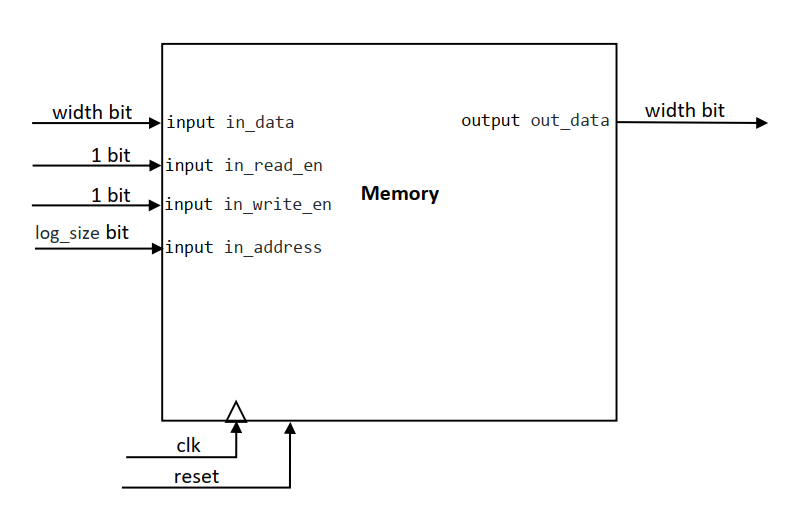
\includegraphics[width=0.5\linewidth]{source/Memory.png}
	\caption{\lr{Memory}}
\end{figure}
	
\subsection{توصیف ماژول‌ها}

\begin{itemize}
	\item 
	\lr{Memory}:
	واحد مموری سخت‌افزار که مطابق با استانداردی که ابتدا آورده شده است. این واحد شامل یک باس خروجی داده است که ماژول‌ها می‌توانند از آن استفاده کنند. همچنین دارای یک باس ورودی و باس آدرس می‌باشد که \lr{Arbiter} تعیین می‌کند که کدام ماژول حق استفاده از این باس ‌ها و همچنین حق استفاده از \lr{enable}های‌ خواندن و نوشتن را دارد.
	\item 
	\lr{Arbiter}
	این واحد نقش پخش کردن اجازه‌ی دسترسی به مموری را بین ماژول‌ها دارد، به \lr{FSM} زیر توجه کنید:
	
\begin{figure}[h]
	\centering
	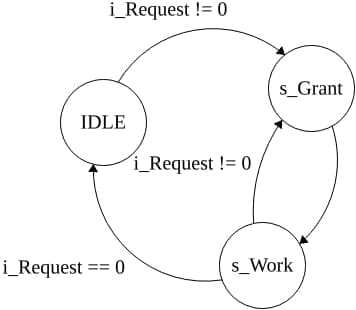
\includegraphics[width=0.35\linewidth]{source/fsm_ar.jpg}
	\caption{\lr{Arbiter Fsm}}
\end{figure}

نحوه‌ی عملکرد این ماژول به این صورت است که یک صف بااهمیت از ماژول‌هایی که آن وصل هستند را نگه می‌دارم و در صورتی که ورودی \lr{Request} آن یک باشد به بااهمیت‌ترین ماژول متصل به خود اجازه‌ی دسترسی به حافظه را می‌دهد. سپس آن ماژول می‌تواند از مموری استفاده کند.
	
	\item 
	\lr{Control Unit}:
	این ماژول وظیفه‌ی محاسبه‌ی حاصل جمع زیر را دارد:
	$$ C_{ij} = \sum_{x=0}^\mu A_{ix}B_{xj} $$
	در واقع این ماژول با پیاده کردن دیاگرام حالت زیر اندیس‌ها را تغییر می‌دهد و هر بار $A_{ix},B_{xj}$ جدید را از حافظه‌ می‌خواند و سپس آن را به واحد ضرب کننده‌ی ماتریسی می‌دهد و پس از اینکه جواب نهایی حاضر شد آن را در حافظه می‌نویسد.
	\begin{figure}[h]
		\centering
		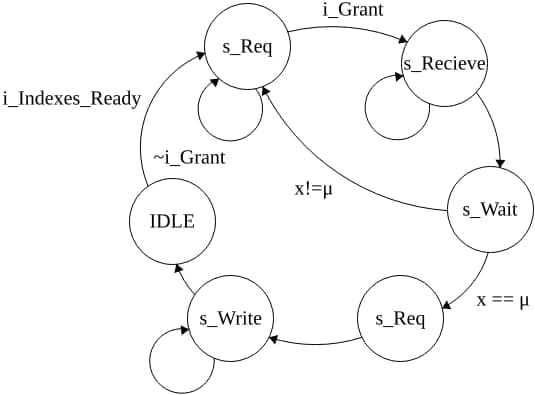
\includegraphics[width=0.4\linewidth]{source/fsm_cu.jpg}
		\caption{\lr{CU Fsm}}
	\end{figure}
توجه می‌کنیم که در حالت \lr{Receive} به اندازه‌ی
 $2k^2$
 باید صبر کنیم تا تمام بیت‌های مورد نیازمان نوشته شود همچنین این حالت به دو حالت درونی \lr{Receive A} و \lr{Receive B} تقسیم بندی می‌شود.
	
	\item 
	\lr{Main Control Unit}:
	این واحد وظیفه‌ی پخش کردن بلاک‌های $C_{ij}$ بین پردازنده‌ها را دارد به نمودار حالت زیر توجه می‌کنیم:
	
	\begin{figure}[h]
		\centering
		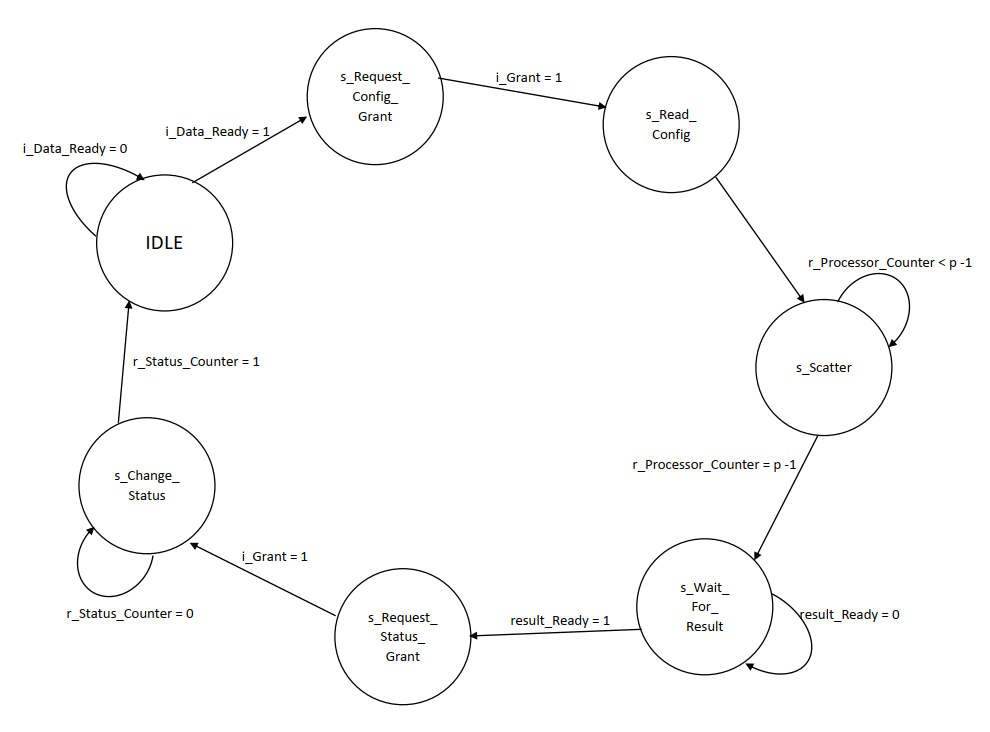
\includegraphics[width=0.4\linewidth]{source/main_cu_fsm.png}
		\caption{\lr{Main CU Fsm}}
	\end{figure}
	
	همان طور که از این نمودار حالت مشخص است هرگاه کلمه‌ی \lr{status} در حافظه نشان‌ دهنده \lr{Cpu\_Ready} باشد از حالت اولیه‌ خارج می‌شویم و از \lr{Arbiter} درخواست می‌کنیم که حافظه‌ را در اختیار ما بگذارد، سپس با داشتن کانفیگ می‌توانیم بین \lr{Processor}‌‌های مختلف اندیس‌ها را پخش کنیم. این کار به اندازه‌ی $\theta$بار انجام می‌دهیم تا نهایتا همه‌ی $C_{ij}$‌ها توسط پردازنده‌ها محاسبه شده و در مموری ذخیره شود. سپس با درخواست از \lr{Arbiter} دسترسی به حافظه را بدست می‌آوریم و کلمه‌ی \lr{status} را تغییر می‌دهیم تا \lr{CPU} متوجه به پایان رسیدن عملیات شود.
	
	\item 
	\lr{Processor Unit}:
	این واحد متشکل از \lr{Control Unit} و \lr{Matrix Multiplier} و \lr{Register File} می‌باشد و وظیفه‌ی برقراری ارتباط بین آنها را دارد. به طور خلاصه این واحد دستورات کنترل یونیت را به مموری می‌فرستد و داده‌ها را درون رجیسترفایل می‌ریزد و یا از آن می‌خواند و \lr{Matrix Multiplier} با استفاده از داده‌های موجود در رجیستر فایل ضرب ماتریسی را انجام می‌دهد و نهایتا خروجی را درون رجیستر فایل می‌ریزد. سپس با استفاده از دستورات واحد کنترلی مقادیر موجود در رجیستر فایل به حافظه انتقال پیدا می‌کند.
	\item 
	\lr{Matrix Multiplier}:
	این واحد وظیفه‌ی ضرب ماتریسی دو ماتریس $k*k$ را دارد به نمودار حالت زیر توجه کنید:
	\begin{figure}[h]
		\centering
		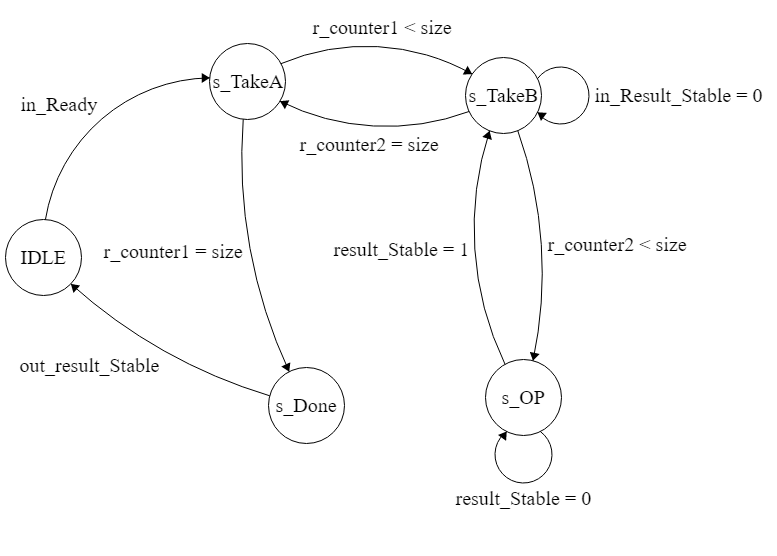
\includegraphics[width=0.5\linewidth]{source/square_matrix.png}
		\caption{\lr{Multiplier Fsm}}
	\end{figure}
	در حالت اول با دریافت بیت \lr{in\_Ready} که از طرف واحد کنترلی می‌آید مشخص می‌شود که باید مراحل ضرب کردن را آغاز کند و این ماژول با استفاده از رجیستر‌های میانی زمان پایان عملیات ضرب را متوجه می‌شود.
	\item 
	\lr{Index To Address Transformer}
	این واحد با داشتن کانفیگ و همچنین ورودی‌های مشخص کننده‌ی دیگر باید بتوانند آدرس $A_{ix}$ یا $B_{xj}$ و یا $C_{ij}$ را پیدا کند بیت‌های ورودی این واحد شامل اندیس سطر و ستون و ۳ بیت دیگر که مشخص می‌کند باید آدرس کدام یک از $A,B,C$ را پیدا کند.
\end{itemize}

\pagebreak
\subsection{ساختار درختی سیستم}

	\begin{figure}[h]
	\centering
	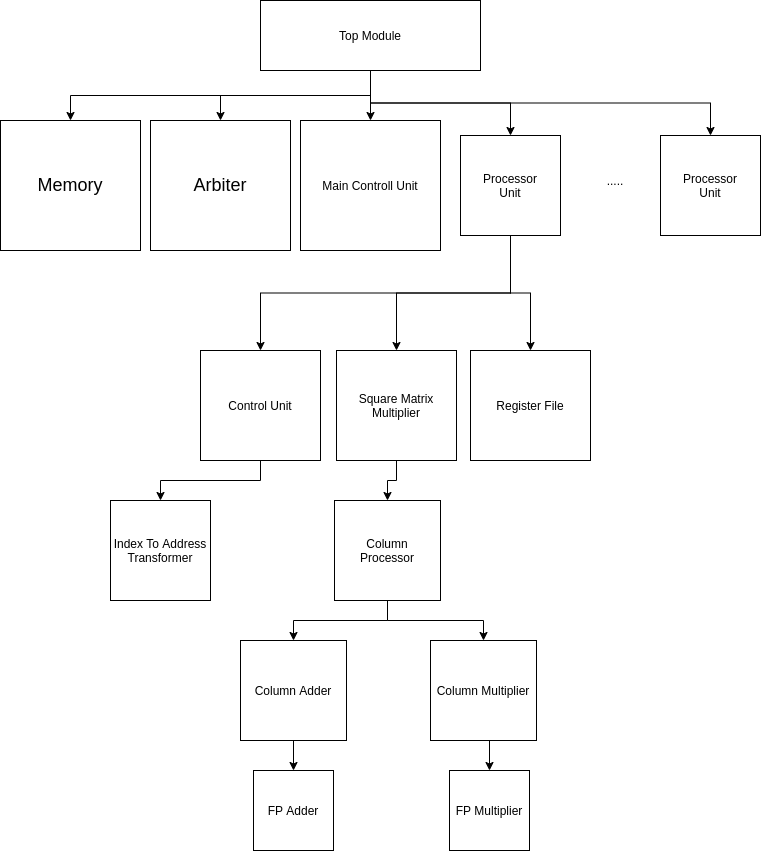
\includegraphics[width=0.87\linewidth]{source/tree.png}
	\caption{\lr{Design Hierarchy}}
\end{figure}

\pagebreak
\section{روند شبیه‌سازی و نتایج حاصل}
\subsection{توصیف \lr{TestBench}ها}
\subsection{توصیف روند کلی شبیه‌سازی}
\subsection{توصیف \lr{Golden Model}}
\subsection{مقایسه‌ی خروجی‌های نهایی با \lr{Golden Model}}



\end{document}







